%
% ======================================================================

\RequirePackage{docswitch}
% \flag is set by the user, through the makefile:
%    make note
%    make apj
% etc.
\setjournal{\flag}

\documentclass[\docopts]{\docclass}

% You could also define the document class directly
%\documentclass[]{emulateapj}

% Custom commands from LSST DESC, see texmf/styles/lsstdesc_macros.sty
\usepackage{lsstdesc_macros}
\usepackage{graphicx}
\graphicspath{{./}{./figures/}}
\bibliographystyle{apj}
\usepackage{subcaption}

% Add your own macros here:
    \usepackage{etoolbox}
    %\usepackage{stackengine}
        \setcounter{secnumdepth}{4}
      \usepackage{csvsimple}
      \usepackage{hyperref}
      \usepackage{adjustbox}
      %\usepackage{float}
      \usepackage{numprint}

%
% ======================================================================

\begin{document}

\title{ LSST Catalog-level Realization of Gravitationally-lensed Quasars }

\maketitlepre

\begin{abstract}

The scale of the LSST dataset will be enormous that we need a different method to classify lensed images of quasars than manually picking the images out. We should anticipate extracting as much information out of its catalogs as possible before ever turning to the pixel-level data. In this work we explore the use of simple, low-multiplicity Gaussian mixture models for realizing gravitational lens systems in LSST catalog space, to enable both large-scale sample simulation and direct model inference.


\end{abstract}

% Keywords are ignored in the LSST DESC Note style:
\dockeys{methods: statistical, cosmology: gravitational lenses}

\maketitlepost

% ----------------------------------------------------------------------

\section{Introduction}
\label{sec:intro}

The Large Synoptic Survey Telescope (LSST), a wide-field survey telescope with the diameter of 8.4m, will start running in Chile in 2020 \cite{LSST_overall}. This telescope has a 3.5 $deg$ of field of view, would cover around 30000 $\textit{deg}^2$ in the sky, and uses $u$, $g$, $r$, $i$, $z$, and $y$ filters \cite{LSSTScienceBookv2}. The telescope will give an extensive amount of astronomical data that could be used for the study of Solar System, Extragalactic structures, near-Earth asteroids, radiant radio sources, Dark Matter, and Dark Energy \cite{LSSTScienceBookv2}. 


LSST Dark Energy Science Collaboration (DESC) also anticipate to detect around 8000 strongly lensed systems that will provide useful information such as cosmological time delay or lens mass distribution \cite{DESC_overall} \cite{TimeDelayOverall} \cite{Twinkles}. Time delay could be used to infer cosmological parameters \cite{Cosmology from Gravitational Lens Time Delays and Planck Data} \cite{Dissecting the Gravitational Lens B1608+656} \cite{Treu2010} which describes the state of the universe.

In order to perform such research, finding the lensed system among the enormous set of data is crucial. However, LSST is also expected to produce 80 terabytes of data each night \cite{LSSTScienceBookv2}.
Considering the amount of the data that LSST will produce, pixel-level searching with images(\cite{RINGFINDER}) may be impossible. In order to solve the problem, we propose the lens classification with catalog-level searching with machine learning techniques (SLRealizer). 

The attempt to use Machine Learning to detect lensed system is not a completely new idea. \citep{convolution_neural_network} suggests that morphological classification of the lensed system using the Convolutional Neural Network(CNN) could be effective. \citep{LensExtractor} has developed 'lensextractor' that uses convolution neural network to train and test the software to detect the lensed system.

The 'SL Realizer' project largely consists of two major parts: finding the useful feature sets to classify the lensed systems from other objects and classifying the lensed systems with different machine learning algorithms.  



\section{Method}
\label{sec:method}

\subsection{Preparation of Data}
\label{subsec:dataprep}

Twinkles, a simulated LSST sky with observed with six filters for ten years, provided the ten years of mock observation history. We also had OM10 mock lensed systems \cite{TimeDelayOverall}. 

We assumed that OM10 mock lensed systems are composed of point-like sources. This means that the size of the galaxies as well as the quasar images had the effective radius of zero.

\begin{table}[!h]
\csvautotabular{../../data/paper_history.csv} %https://texblog.org/2012/05/30/generate-latex-tables-from-csv-files-excel/ %bug
\caption{Few entries of the twinkles mock observation history data. Full data can be accessed \href{https://github.com/jennykim1016/SLRealizer/blob/master/data/twinkles_observation_history.csv}{here}.}
\end{table}

In order to save some computation time, we queried the first three years of the observation which yields 263 observation epochs. We also selected LSST-like OM10 mock lensed systems by querying with magnitude cut of 22.5. 

% ----------------------------------------------------------------------

\section{Data Preparation}
\label{sssec:catalog}
\subsection{Toy Source Catalog}

\label{sssec:toysource}

Using the data from \ref{subsec:dataprep}, we were able to make an each entry of catalog describing how each lensed system would look like on a particular night. While doing this, we assumed that all the sources in the lensed system have Gaussian point spread functions. Also, we realized the systems with a null-deblender, meaning that we assumed that all the lensed images and the lens were observed as one big source.

In order to do so, we used Galsim package in Python. For each lensed system, we drew a Gaussian that has an effective radius of a galaxy as well as adding the rotation angle and shears to the values. We also drew the Gaussians that have an effective radius of zero in the position for the quasar images. Then, we convolved the Gaussians with the Gaussian point spread functions. After then, we added all the convolved Gaussian onto the two-dimensional grid that has the same degree-to-pixel ratio (0.2 arcseconds per pixels) as LSST, realizing the total sum as one Gaussian. After the realization, we could get ellipticity, zeroth moment, the first moment, and the second moment per one big convolved Gaussian.
\begin{figure}
    \centering
    \begin{subfigure}[bt]{0.48\linewidth}        %% or \columnwidth
        \centering
        
\includegraphics[width=\linewidth, height=8cm]{beforenulldeblend.png}
        \caption{Before null-deblending, the whole system looks like this image. The brightest source is the lensing galaxy, and there are two dimmer quasar images near the galaxy. There is only one quasar images that are obvious that makes the image more elliptical.}
    \end{subfigure}
    \begin{subfigure}[bt]{0.48\linewidth}        %% or \columnwidth
        \centering
        
\includegraphics[width=\linewidth, height=8cm]{afternulldeblend.png}
        \caption{After null-deblending, the whole system looks like this image. All the sources look like one big source observed at once.                                                                                                                                                                                 }
    \end{subfigure}
    \caption{Example null-deblending.}
    \label{fig:null-deblend}
\end{figure}

The toy catalog is in \ref{sssec:toysource}.

\subsection{Toy Object Catalog}
\label{sssec:toyobject}

After generating the source catalog, we computed the object table whose entree describes average properties of each lensed system per filter. In order to do so, we queried each lensed system in the source catalog. Then, for each lensed system, we computed the average properties for each filter.

The toy catalog is in \ref{subsec:toyobject}.

\subsection{Feature Selection}
\label{subsec:feature}

For now, we focused on classifying the lensed systems from the SDSS galaxies. We expect the lensed images to appear near the bright, massive galaxies. Thus, if we can differentiate the galaxies with lensed images with the galaxies without them, it would be really helpful.

We expect that the quasar images will be brighter in the shorter wavelength filters. The galaxies will be brighter in the longer wavelength filters. Thus, when we observe a lensed system through a $u$ filter (the shortest wavelength filter that OM10 has), we will see the more stretched object because of the contribution from the quasar images. However, in the $z$ band, we will see a round object because of the contribution from the lens. By comparing the features in the $u$ filter and the $z$ filter, we will thus be able to see bigger changes in the properties for the lensed systems than SDSS galaxies.

The features that we could get from the object table is changes in the first moment along the x-axis (reference to the $r$ filter), changes in the first moment along the y-axis (reference to the $r$ filter), changes in the position (reference to the $r$ filter), ellipticities, rotation angles, fluxes, and sizes.

The catalog of SDSS galaxies also provides the same features. Magnitude systems are the same in both SDSS and OM10, and the units are scaled to be the same. However, the only difference was in the sizes. SDSS's definition of size was $I_{xx}$ + $I_{yy}$. Galsim calculates the size of OM10 systems by calculating the determinant of the second moment(M $=$ $I_{xx}$ * $I_{yy}$ - $I_{xy}$ * $I_{xy}$) and applying the fourth root on it ($\sqrt[4]{M}$). In order to solve the problem by scaling the SDSS sizes, we multiplied the power of pixel-to-arcsec ratio to change the unit to arcseconds, multiplied two to convert the half size to the full size, and applied the square root to the value to get a right dimension.

Using these values, we computed various additional features. We plotted SDSS galaxies and OM10 lensed systems onto the corner plot \ref{subsec:feature}, and chose the features that differentiated OM10 lensed systems from SDSS galaxies the most.

\subsection{Classification}
\label{subsec:classification}

We have 2323 OM10 lensed systems and 16000 SDSS galaxies. In order to make the balanced test data set, we randomly selected 2323 SDSS galaxies. We mixed the order of those two samples so that there will be a roughly same number of each OM10 and SDSS samples in both the test and the training data. Then, using the scikit train$\_$test$\_$split method, we selected 75$\%$ of the data to be the training set and performed the test on the remaining 25$\%$.

According to the scikit's \href{http://scikit-learn.org/stable/tutorial/machine_learning_map/index.html} {choosing the right estimator}, we were able to choose three different algorithms for the classification purposes. We did have more than 50 samples, we were predicting a category, we did have a labeled data, and we had less than 100K samples in a text data. This yields Linear SVC, KNeighbors Classifier, and Ensemble classifiers such as Random Forest.

Detailed results are in \ref{subsec:classification_data}.

% ----------------------------------------------------------------------

\section{Results}
\label{sec:results}

\subsection{Toy Source Catalog}
\label{subsec:toysource}

\begin{table}[!h]
\centering
\begin{tabular}{|l|l|l|l|l|l|l|l|l|l|l|}
\hline
lensid   & MJD          & filter & RA & RA\_err & DEC & DEC\_err & x              & x\_com\_err & y               & y\_com\_err \\ \hline 
710960   & 59823.286523 & g      & 0  & 0       & 0   & 0        & 2.1350  & 0           & 1.2151 & 0			\\
17432684 & 59823.286523 & g      & 0  & 0       & 0   & 0        & 0.1226 & 0           & 0.7593  & 0           \\
50310149 & 59823.286523 & g      & 0  & 0       & 0   & 0        & 0.2527 & 0           & 0.4665  & 0           \\
52812164 & 59823.286523 & g      & 0  & 0       & 0   & 0        & 0.3874 & 0           & -0.3413 & 0          \\ \hline
\end{tabular}
\begin{tabular}{|l|l|l|l|l|l|l|l|l|l|}
\hline
flux          & flux\_err       & size          & size\_err & e1               & e2                & e               & phi             & psf\_sigma & sky       \\ \hline
21.9127 & 0.03549 & 1.4501 & 0         & 0.2386    & 0.3360    & 0.4121  & 0.4766  & 1.093153   & 24.377204 \\
18.2072 & 0.03549& 1.1802  & 0         & -0.0550 & -0.004712  & 0.05525 & 0.04270 & 1.093153   & 24.377204 \\
5.9831 & 0.03549 & 1.2253 & 0         & -0.05931 & 0.02588     & 0.06471 & -0.2057 & 1.093153   & 24.377204 \\
6.2727 & 0.03549 & 1.2102  & 0         & -0.03114 & -0.05654  & 0.06455 & 0.5336  & 1.093153   & 24.377204 \\ \hline
\end{tabular}
\caption{Few sample entrees of the toy source catalog. The full toy object catalog can be viewed \href{https://www.dropbox.com/s/muqui8eu3kxox2l/toy_source_catalog.csv?dl=0}{here}}
\label{table:source_table}
\end{table}

The above is the toy source catalog that we generated. For now, we haven't added error terms and calculated the positions (RA and DEC).

\subsection{Toy Object Catalog}
\label{subsec:toyobject}

\begin{table}[!h]
\centering

\begin{tabular}{|l|l|l|l|l|l|l|l|l|l|l|l|l|}
\hline
lensid     & u\_flux & u\_x   & u\_y   & u\_size & u\_flux\_err & u\_x\_com\_err & u\_y\_com\_err & u\_size\_err & u\_e1   & u\_e2   & u\_e   & u\_phi \\ \hline
710960.0   & 37.0846 & 2.2817 & 1.2996 & 1.4151  & 0.2511       & 0.0            & 0.0            & 0.0          & 0.1399  & 0.205   & 0.2496 & 0.4574 \\ \hline
17432684.0 & 26.7018 & 0.1211 & 0.7633 & 0.971   & 0.2516       & 0.0            & 0.0            & 0.0          & -0.0968 & -0.0092 & 0.0972 & 0.0497 \\ \hline
\end{tabular}

\begin{tabular}{|l|l|l|l|l|l|l|l|l|l|ll|}
\hline
g\_flux & g\_x   & g\_y   & g\_size & g\_flux\_err & g\_x\_com\_err & g\_y\_com\_err & g\_size\_err & g\_e1   & g\_e2   & g\_e   & g\_phi	\\ \hline
19.9485 & 2.1555 & 1.2328 & 1.4608  & 0.1244       & 0.0            & 0.0            & 0.0          & 0.1967  & 0.2768  & 0.3395 & 0.4765 \\ \hline
17.5991 & 0.1221 & 0.7518 & 1.2413  & 0.1244       & 0.0            & 0.0            & 0.0          & -0.0532 & -0.0045 & 0.0534	& 0.0425	\\ \hline
\end{tabular}


\begin{tabular}{|l|l|l|l|l|l|l|l|l|l|l|l|}
\hline
r\_flux & r\_x   & r\_y   & r\_size & r\_flux\_err & r\_x\_com\_err & r\_y\_com\_err & r\_size\_err & r\_e1   & r\_e2   & r\_e   & r\_phi \\ \hline
31.0886 & 2.27   & 1.2928 & 1.2608  & 0.0923       & 0.0            & 0.0            & 0.0          & 0.1693  & 0.2395  & 0.2933 & 0.4779 \\
25.2258 & 0.1215 & 0.7617 & 0.9958  & 0.0923       & 0.0            & 0.0            & 0.0          & -0.0867 & -0.0078 & 0.087  & 0.0457 \\ \hline
\end{tabular}

\begin{tabular}{|l|l|l|l|l|l|l|l|l|l|l|l|}
\hline
i\_flux & i\_x   & i\_y   & i\_size & i\_flux\_err & i\_x\_com\_err & i\_y\_com\_err & i\_size\_err & i\_e1   & i\_e2   & i\_e   & i\_phi \\ \hline
26.2547 & 2.3012 & 1.3075 & 1.2154  & 0.0433       & 0.0            & 0.0            & 0.0          & 0.1521  & 0.2146  & 0.263  & 0.4773 \\
22.747  & 0.1217 & 0.7612 & 1.0063  & 0.0433       & 0.0            & 0.0            & 0.0          & -0.0813 & -0.0071 & 0.0816 & 0.0436 \\ \hline
\end{tabular}

\begin{tabular}{|l|l|l|l|l|l|l|l|l|l|l|l|}
\hline
z\_flux & z\_x   & z\_y   & z\_size & z\_flux\_err & z\_x\_com\_err & z\_y\_com\_err & z\_size\_err & z\_e1   & z\_e2   & z\_e   & z\_phi \\ \hline
19.7955 & 2.264  & 1.2879 & 1.2545  & 0.0322       & 0.0            & 0.0            & 0.0          & 0.1595  & 0.2247  & 0.2755 & 0.4767 \\
18.0387 & 0.1216 & 0.7587 & 1.0622  & 0.0315       & 0.0            & 0.0            & 0.0          & -0.0751 & -0.0064 & 0.0754 & 0.0426 \\ \hline
\end{tabular}

\caption{Few sample enrees of the toy object catalog. The full toy object catalog can be viewed \href{https://www.dropbox.com/s/ob51rxjexzuervl/toy_object_catalog.csv?dl=0}{here}}
\label{table:object_table}
\end{table}

\ref{table:object_table} is the toy object catalog that we generated.

\subsection{Feature Selection}
\label{subsec:feature_data}

Full corner plots can be viewed in the \href{https://github.com/jennykim1016/SLRealizer/blob/master/notebooks/SDSSvsOM10.ipynb}{SLRealizer's GitHub repository's notebook folder}.

As mentioned in \ref{subsec:feature}, we thought comparing features between $u$ and $z$ filter will be discriminatory. We chose six main features that we thought would change dramatically between the filters for OM10 lenses -- sizes, ellipticities (e), rotation angles of galaxies ($\phi$), magnitudes, positions($\Delta$ x), and the angle between ellipticity vector and the rotation vector ($\omega = \frac{e \cdot \phi}{ \left | e \right | \left | \phi \right |}$).

\begin{figure}
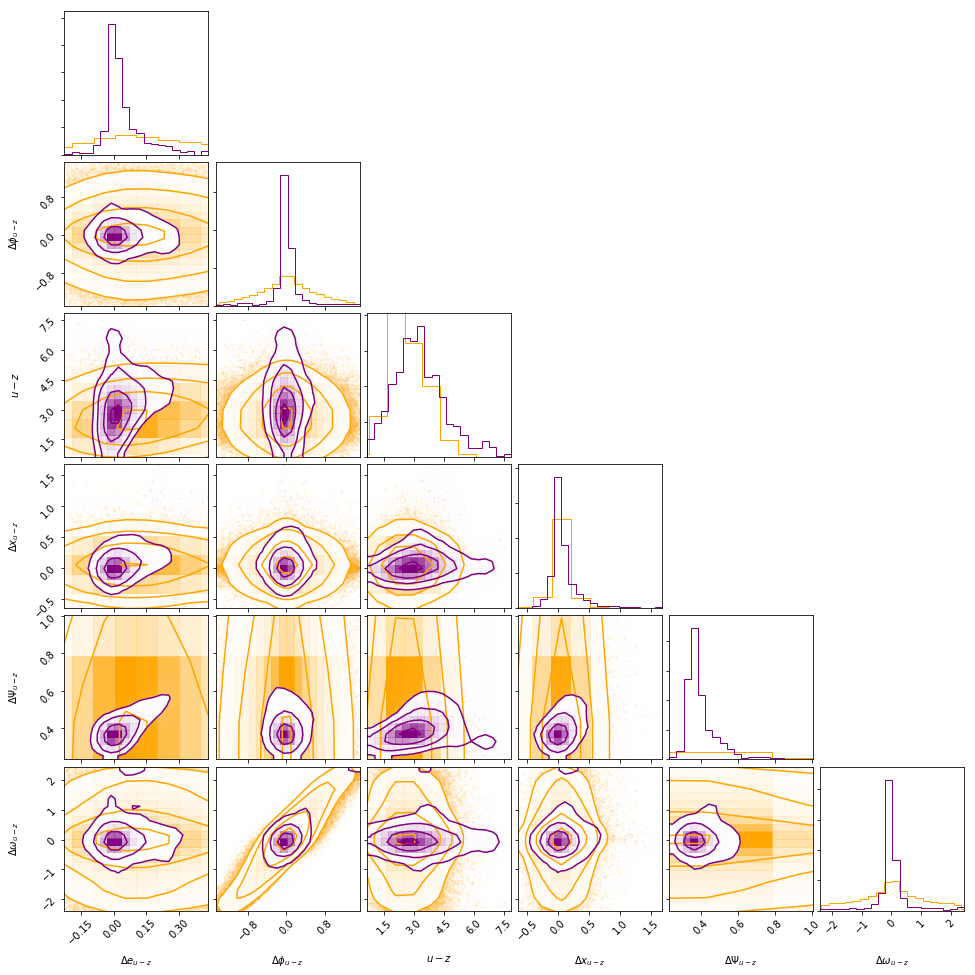
\includegraphics[width=0.9\columnwidth]{cornerplot.png}
\caption{The cornerplot with six features.}
 \label{fig:cornerplot}
\end{figure}

Here, the centroid of the yellow points(SDSS galaxies) and the purple points(OM10 systems) differed the most for size. Still, we could quantify the importance of the features by putting all the data into the Random Forest Algorithms. The results were as follows.

\begin{figure}[!h]
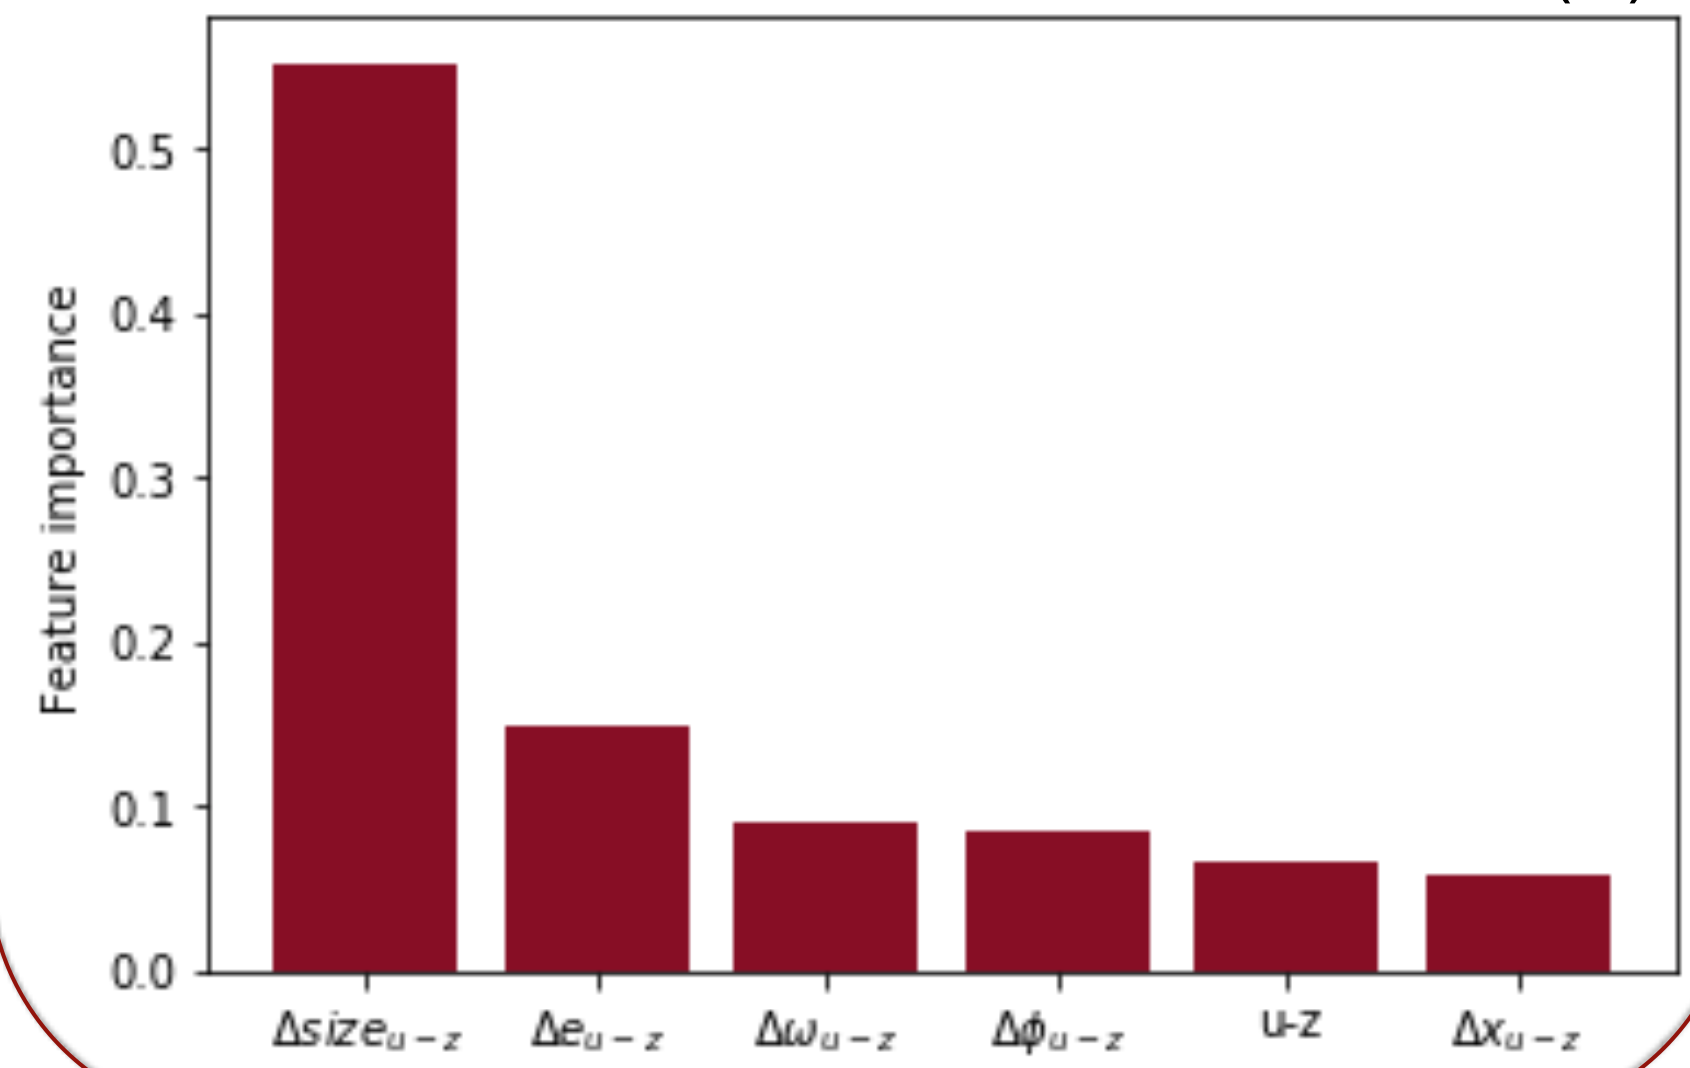
\includegraphics[width=0.4\columnwidth]{FeatureImportance.png}
\caption{Feature importance calculated with the Random Forest algorithm.}
 \label{fig:featureimportance}
\end{figure}

\subsection{Classification}
\label{subsec:classification_data}

As mentioned in \ref{subsec:classification}, we used three different algorithms: linear SVC, KNeighbors (Nearest Neighbors), and Random Forest. \ref{fig:ML_nonmag} is the results that we got for each algorithm.

Random forest showed the best performance among the three different algorithms. If we look into the top left corner where all the curves are overlapped, we can see this more obviously. The best classifiers were Random Forest, and the more the number of estimators were, the better the algorithm performed. For the best algorithm, we were able to achieve ~98$\%$ of the true positive rate(TPR) and ~0.04$\%$ of the false positive rate(FPR).

\begin{figure}
    \centering
    \begin{subfigure}[bt]{0.48\linewidth}        %% or \columnwidth
        \centering
        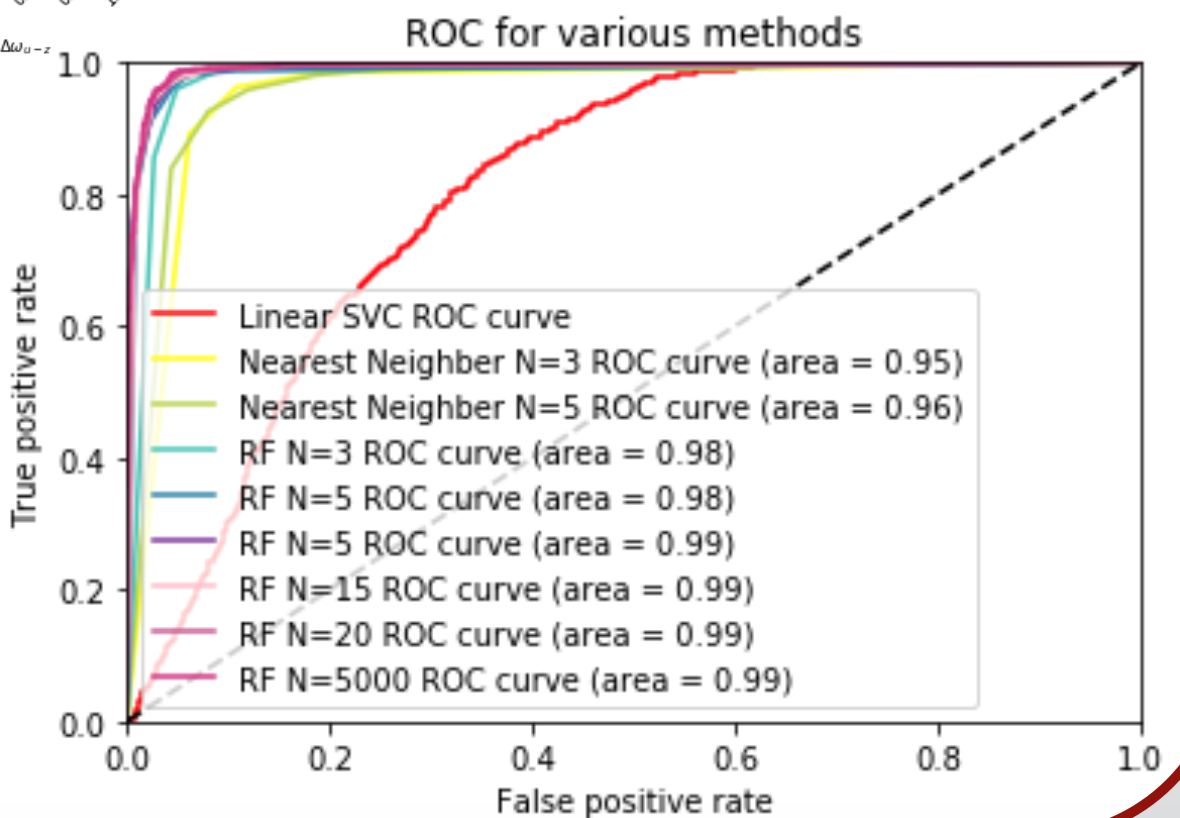
\includegraphics[width=\linewidth]{ML_notmagnified.png}
    \caption{ROC curve for each algorithm}
     \label{fig:ML_nonmag}
    \end{subfigure}
    \begin{subfigure}[bt]{0.48\linewidth}        %% or \columnwidth
        \centering
        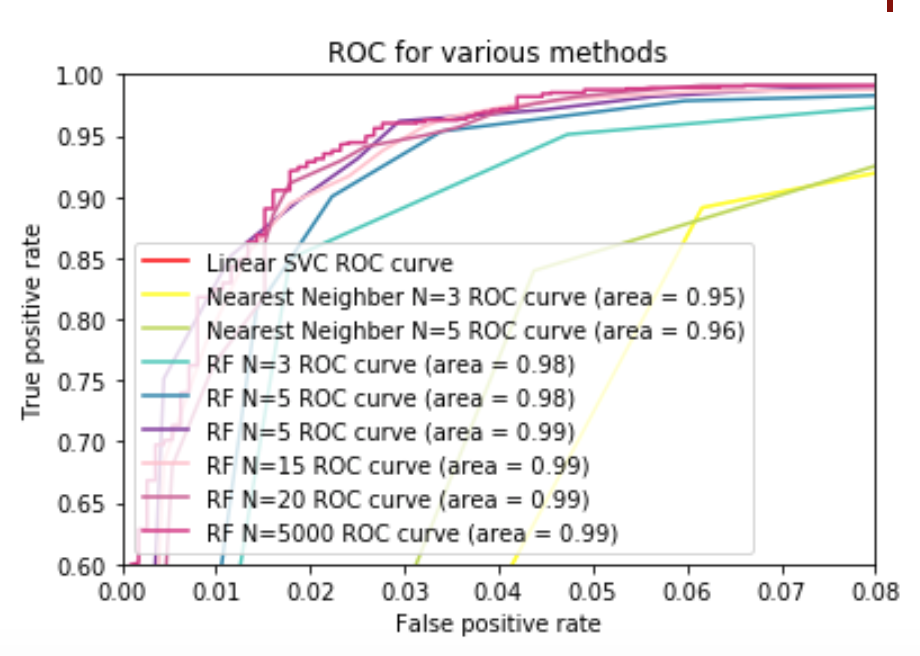
\includegraphics[width=\linewidth]{ML_magnified.png}
        \caption{ROC curve from FPR (0, 0.08) and TPR (0.6, 1.0)}
         \label{fig:ML Magnified}
    \end{subfigure}
    \caption{Example null-deblending.}
    \label{fig:null-deblend}
\end{figure}

% ----------------------------------------------------------------------

\section{Conclusions}
\label{sec:conclusions}

The results suggest that random forest algorithms would be able to differentiate lensed systems from galaxies. Still, even though we have high accuracy, because we expect to have much more non-lensed systems than the lensed systems, we will have more contaminants in the truly-classified lensed systems than the actual lensed systems. For instance, we expect to find 10,000 times more non-lensed systems than the lensed ones. Thus, with 98\% of the TPR and ~0.042\% of the FPR, we will have ~430 contaminants per truly classified lensed systems. Thus, it would also be helpful to have a more rigorous model that actually fits physical models to the systems after rejecting all the non lensed-systems using SLRealizer.

In addition, we only compared the features between OM10 lensed systems and SDSS galaxies. It will also be useful to overlap star-star pairs, star-galaxy pairs, quasar-quasar pairs, or quasar-galaxy pairs to see how different the other samples could be from the lensed system.

There are few ways to further improve the classifiers. If we could implement the working deblender that resembles LSST’s deblender, that will increase the performance of the classifiers. We could also add more features such as time-variabilities of quasar images. While making the source and the object catalog, rather than giving equal weights to all the observations, we could weight by how good the seeing was for each night.

In addition, while studying cosmology, gravitationally lensed systems with four images (quads) are generally more useful than the systems with two images (doubles). Thus, comparing how many quads were classified as true out of the testing sample’s quads should also give useful measures.

% ----------------------------------------------------------------------
% GUIDELINES FROM THE NOTE TEMPLATE:
%
% \section{Introduction}
% \label{sec:intro}
%
% This is a paper and note template for the LSST DESC \citep{Overview,ScienceBook,WhitePaper}.
% You can delete all this tutorial text whenever you like.
%
% You can easily switch between various \LaTeX\xspace styles for internal notes and peer reviewed journals.
% Documents can be compiled using the provided \code{Makefile}.
% The command \code{make} with no arguments compiles \code{main.tex} using the  \code{lsstdescnote.cls} style.
% If you want to upgrade your Note into a journal article, just choose a journal name, between \code{make apj} (ApJ preprint format), \code{make apjl} (which uses the \code{emulateapj} style), \code{make prd}, \code{make prl}, and \code{make mnras}.
%
%
% % ----------------------------------------------------------------------
%
% \section{Commands}
% \label{sec:commands}
%
% There are a number of useful \LaTeX\xspace commands predefined in \code{macros.tex}.
% Notice that the section labels are prefixed with \code{sec:} to allow the use of the \verb=\secref= command to reference a section (\ie, \secref{intro}).
% Figures can be referenced with the \verb=\figref= command, which assumes that the figure label is prefixed with \code{fig:}.
% In \figref{example} we show an example figure.
% You'll notice that the actual figure file is found in the \code{figures} directory.
% However, because we have specified this directory in our \verb=\graphicspath= we do not need to explicitly specify the path to the image.
%
% The \code{macros.tex} package also contains some conventional scientific units like \angstrom, \GeV, \Msun, etc. and some editorial tools for highlighting \FIXME{issues}, \CHECK{text to be checked}, \COMMENT{comments}, and \NEW{new additions}.
%
%
% % ----------------------------------------------------------------------
%
% \section{Methods}
% \label{sec:methods}
%
% Similar to the figure before, here we have included a table of data from \code{tables/table.tex}.
% Notice that again we are able to reference \tabref{example} with the \verb=\tabref= command using the \code{tab:} prefix.
% Also notice that we haven't needed to specify the full path to the table because in the \code{Makefile} we include \code{./tables} directory in the \code{\$TEXINPUTS} environment variable.
%
% \begin{table}
  \begin{center}
  \caption{Example table. \label{tab:example}}
  %\begin{ruledtabular}
  \begin{tabular}{lccc}
\hline\hline
Column 1 & Column 2 & Column 3 &  Column 4 \\[3pt]  
     &    $\deg$     & $\kpc$   &  $\deg$ \\[4pt]
\hline
Obj1 & (0,0) & 10 & 0.1 \\
... & ... & ... & ... \\
ObjN & (0,0) & 10 & 0.1
\\\hline\hline
\end{tabular}
\end{center}
%\end{ruledtabular}
\end{table}

%\begin{\tabletype}{l ccccccc }
%\tablewidth{0pt}
%\tabletypesize{\tiny}
%\tablecaption{ An example table. \label{tab:example}}
%\tablehead{
%(1) & (2) & (3) & (4) & (5) & (6) & (7) & (8)\\
%Name & GLON,GLAT & Distance & $r_{1/2}$ & $\log_{10}(J_{\rm meas})$ & $\log_{10}(J_{\rm pred})$ & Sample & Refrence \\
% & (deg) & (kpc) & (pc) & $\log_{10}(\GeV^2 \cm^{-5})$ & $\log_{10}(\GeV^2 \cm^{-5})$ & & 
%}
%\startdata
%Bootes I                     & 358.08,69.62   & 66  & 189  & $18.8 \pm 0.2$ & 18.5           & I,S,C & ... \\
%\\
%...\\
%\\
%Willman 1                    & 158.58,56.78   & 38  & 19   & $19.1 \pm 0.3$ & 18.9           & I,S & ... \\
%\enddata
%{\footnotesize \tablecomments{ (1) The first column. (2) The second column ...}}
%\end{\tabletype}

%
% Equations appear as follows, and can be referred to as, for example, \eqnref{example} -- just as for tables, we use the \verb=\eqnref= command using the \code{eqn:} prefix.
% \begin{equation}
%   \label{eqn:example}
%   \langle f(k) \rangle = \frac{ \sum_{t=0}^{N}f(t,k) }{N}
% \end{equation}
%
%
% % ----------------------------------------------------------------------
%
% \section{Results}
% \label{sec:results}
%
% \figref{example} shows an example figure, referred to with the \verb=\figref= command and the \code{fig:} prefix.
%
% \begin{figure}
% 
\includegraphics[width=0.9\columnwidth]{example.png}
% \caption{An example figure: the LSST DESC logo, copied from \code{texmf/logos/desc-logo.png} into \code{figures/example.png}. \label{fig:example}}
% \end{figure}
%
%
% % ----------------------------------------------------------------------
%
% \section{Discussion}
% \label{sec:discussion}
%
% If you are planning on committing your paper to GitHub, it's a good idea to write your tex as one sentence per line.
% This allows for an easier \code{diff} of changes.
% It also makes sense to think of latex as \emph{code}, and sentences as logical statements, occupying one line each.
% Each line must ``compile'' in the mind of the reader.
%
%
%
% ----------------------------------------------------------------------

\subsection*{Acknowledgments}

Here is where you should add your specific acknowledgments, remembering that some standard thanks will be added via the \code{acknowledgments.tex} and \code{contributions.tex} files.

% 
This is the text imported from \code{acknowledgments.tex}, and will be replaced by some standard LSST DESC boilerplate at some point.
% 


%Author contributions are listed below. \\
Jenny Kim: Initial algorithm and code development, wrote paper. \\
Ji Won Park: Improved algorithm and code development, edited paper. \\
Phil~Marshall: Initiated  project, advised on motivation, model construction and testing. \\
Mike~Baumer: Advised on LSST data characteristics, model construction and testing. \\
Steve~Kahn: Advised on LSST data characteristics, model construction and testing. \\
Rahul~Biswas: Advised on LSST observing cadence, catalog characteristics, error model. \\


%{\it Facilities:} \facility{LSST}
% Include both collaboration papers and external citations:
\bibliography{lsstdesc,main}

\end{document}
% ======================================================================
%
